% Provenance (jamais imprimé) : voir sources/outline_sources.md (Année 2 : méthodes de terrain et de laboratoire ---
% pétrographie ignée et métamorphique, analyse chimique par XRF, ICP-MS et microsonde, spectrométrie de masse isotopique, une
% campagne de cartographie). Modelé sur le livre 3, ch. 6.
% Textures : BGS RR 99-02 (Robertson 1999), Open University Virtual Microscope, Carleton BH250,
% UCSB Geology 102C (Hacker) ; QAPF : BGS RR 99-06 (Gillespie et Styles 1999) ; instruments : fiches SERC
% Geochemical Instrumentation and Analysis (EPMA, WDS, XRF, TIMS, MC-ICPMS) ; procédure XRF et résultats des
% matériaux de référence : USGS OFR 02-223 et son chapitre T (Taggart et Siems 2002) ; isotopes du Sr :
% CIAAW ; traceur et biais de masse : Cheong, Jeong et Kwon (2014). Lignes du registre dans
% sources/ledger/book4.md ; courbes et stations depuis figdata/bachelor-2/labmethods.py, nombres depuis
% le calculateur de travail du second rédacteur du livre 4 calc/ch31.py. Observation seule : le travail
% professionnel est décrit à la troisième personne.
\chapter{Méthodes de terrain et de laboratoire II}\label{ch:b2:field-lab-methods-2}

Chaque nombre des chapitres de pétrologie de ce livre a commencé par une roche dans un sac, une lame mince sous
un microscope et une poudre dans un instrument. Une composition minérale reportée sur un diagramme de phases, la
teneur en silice qui nomme une lave, le rapport isotopique du strontium qui trace une source mantellique : chacun
est sorti d'une chaîne d'opérations commencée à un affleurement, et chacun porte les erreurs de chaque maillon.
Ce chapitre suit cette chaîne pour les roches du socle des collines de Varden : lire les textures en lame mince,
compter les minéraux, analyser la roche totale, puis des minéraux isolés, puis les isotopes, en se demandant à
chaque étape la qualité du nombre obtenu.

\begin{recall}
\textbf{Du volume de première année}~: station de terrain, carnet de terrain, échantillon orienté, lame mince,
microscope polarisant, lumière polarisée plane, polariseurs croisés ; identification optique des minéraux
formateurs de roches ; recalcul d'une formule minérale à partir d'une analyse en oxydes sur un nombre fixé
d'oxygènes, et du fer ferrique par la neutralité de charge ; foliation et schistosité ; isochrone, rapport
initial et droite des moindres carrés. \textbf{Des livres de chimie}~: spectrométrie de masse, plasma à
couplage inductif ; courbe d'étalonnage, limite de détection, limite de quantification, justesse, biais,
répétabilité, écart type de la moyenne. \textbf{Des livres de physique}~: rayons X caractéristiques et loi de
Moseley ; loi de Bragg ; tension superficielle ; propagation des incertitudes.
\textbf{Des livres de mathématiques}~: loi binomiale, son espérance et sa variance.
\textbf{Du \cref{ch:b2:magmatic-series}}~: \omterm{def:b2:magmatic-series:qapf}{composition modale}, \omterm{def:b2:magmatic-series:qapf}{diagramme QAPF}.
\textbf{Du \cref{ch:b2:isotope-geochemistry}}~: \omterm{def:b2:isotope-geochemistry:tracer}{traceur isotopique radiogénique}, \omterm{def:b2:isotope-geochemistry:standards}{étalon isotopique de référence}.
\end{recall}

\section{Pétrographie : les textures comme une histoire}\label{sec:b2:field-lab-methods-2:petrography}

Le volume de première année utilisait le microscope polarisant pour identifier les minéraux. Le pétrographe lit
aussi la manière dont les grains sont disposés, car cette disposition enregistre l'ordre dans lequel ils ont
crû. Deux textures sont les témoins les plus courants d'une cristallisation à partir d'un \omterm{def:b2:magma-emplacement:magma}{liquide silicaté} et
d'une recristallisation à l'état solide.

\begin{definition}[Texture ophitique, texture granoblastique]\label{def:b2:field-lab-methods-2:textures}
Une roche ignée présente une \emph{texture ophitique}\index{texture ophitique} lorsque de grands cristaux de pyroxène
enferment de petites lattes de plagioclase orientées au hasard ; la texture est typique de la dolérite, du gabbro
et du basalte. Une roche métamorphique présente une \emph{texture granoblastique}\index{texture granoblastique} lorsqu'elle est
un agrégat de cristaux à peu près équidimensionnels, de taille à peu près égale, souvent xénomorphes, dont les
joints droits se rejoignent par trois avec des angles voisins de \ang{120}.
\end{definition}
% ledger: carletonB:ophitic, ouVM:textures, bgsM:textures

Dans une roche ophitique, les lattes enclavées sont entières et automorphes, et le pyroxène remplit l'espace
entre elles~: le plagioclase a cristallisé le premier, le pyroxène autour de lui. Les angles de \ang{120} d'une \omterm{def:b2:field-lab-methods-2:textures}{texture
granoblastique} sont ceux de grains qui ont eu le temps d'ajuster leurs joints~; la littérature pédagogique en pétrographie
interprète de telles jonctions triples comme le signe d'un équilibre chimique et textural. L'angle résulte d'un équilibre des forces, les joints de grains tirant sur leur
ligne commune comme des films de savon (tension superficielle, des livres de physique).
% ledger: ouVM:equilibrium

\begin{proposition}[Angles à une jonction triple]\label{prop:b2:field-lab-methods-2:triple}
Soient trois joints de grains qui se rejoignent le long d'une ligne, de tensions (énergies par unité d'aire) $\gamma_1$,
$\gamma_2$, $\gamma_3$, et soit $\theta_i$ l'angle entre les deux joints autres que
le joint $i$. À l'équilibre,
\begin{equation}
\frac{\gamma_1}{\sin\theta_1} = \frac{\gamma_2}{\sin\theta_2} = \frac{\gamma_3}{\sin\theta_3},
\label{eq:b2:field-lab-methods-2:lami}
\end{equation}
et trois tensions égales se rejoignent sous trois angles de \ang{120}.
\end{proposition}

\begin{proof}
Dans un plan perpendiculaire à la jonction, chaque joint tire la jonction le long de sa propre trace
avec la force $\gamma_i$ par unité de longueur. À l'équilibre les trois forces s'annulent, si bien que, placées
bout à bout, elles forment un triangle fermé. L'angle du triangle opposé au côté $\gamma_i$ vaut
$\pi - \theta_i$, dont le sinus est $\sin\theta_i$, et la loi des sinus dans le triangle donne
\eqref{eq:b2:field-lab-methods-2:lami}. Si les trois tensions sont égales, le triangle est
équilatéral, chaque angle extérieur $\theta_i$ vaut $\pi - \pi/3 = 2\pi/3$, soit \ang{120}.
\end{proof}

\begin{omfigure}
\centering
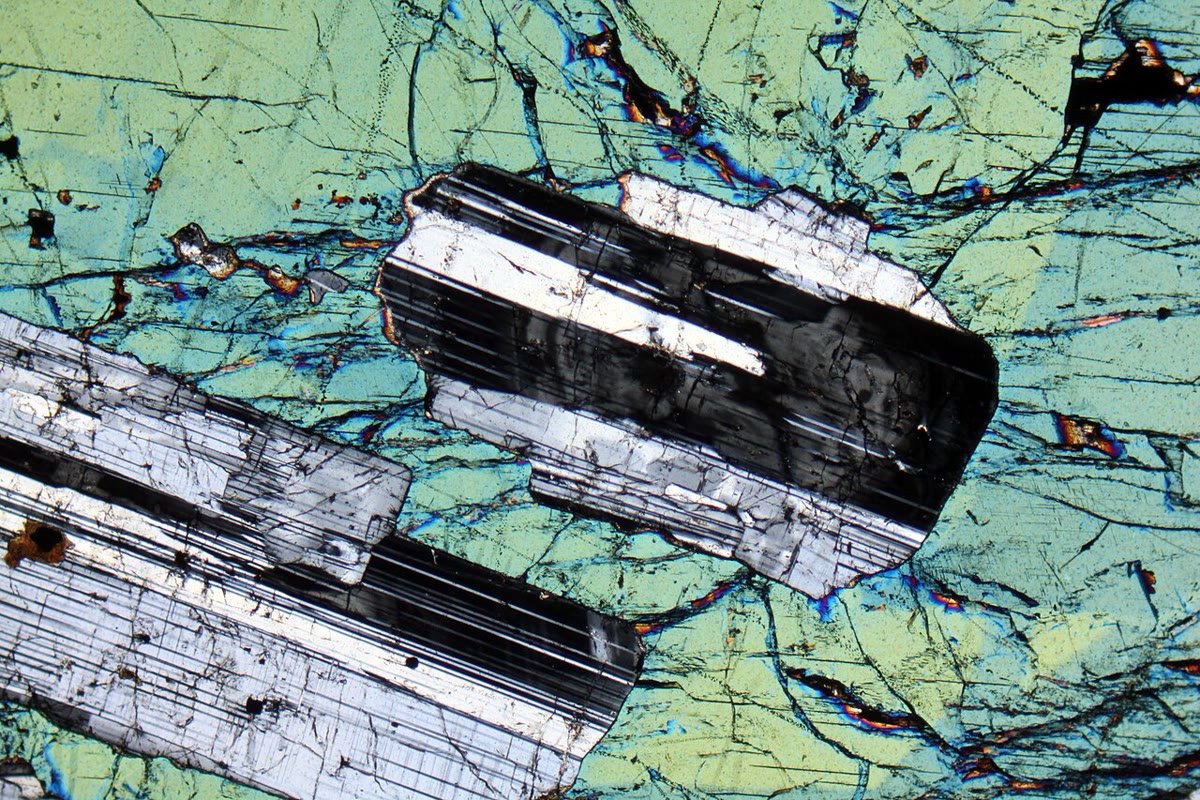
\includegraphics[height=4.6cm]{images/book4/b2-31-ophitic.jpg}\quad
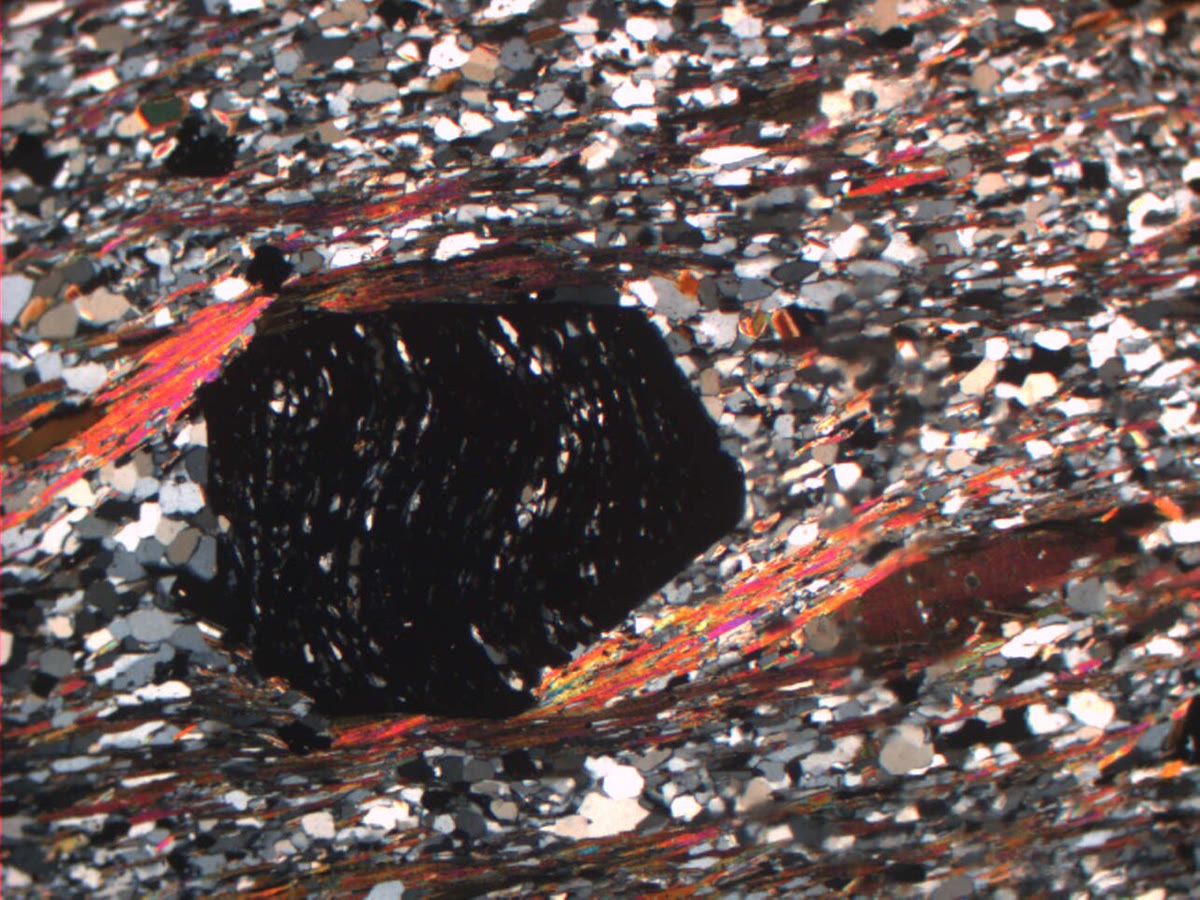
\includegraphics[height=4.6cm]{images/book4/b2-31-garnet-porphyroblast.jpg}
\par\smallskip{\small Deux textures entre polariseurs croisés. À gauche~: un cristal unique d'augite (bleu
et vert) enferme des lattes de plagioclase maclées, disposition propre à une \omterm{def:b2:field-lab-methods-2:textures}{texture ophitique}~; champ de vue \qty{7}{mm}.
Photographie Strekeisen, CC BY-SA 4.0 (Wikimedia Commons). À droite~: un schiste à grenat et mica.
Le grenat, noir car isotrope, est un grand cristal qui a crû à l'état solide~; des inclusions de quartz
le traversent en traînées, et la foliation de la muscovite (couleurs vives), de la biotite (brune) et du quartz
(gris) s'incurve autour de lui.
Photographie Jackdann88, CC BY 3.0 (Wikimedia Commons).}
\end{omfigure}
% ledger: photo:b2-31-ophitic, photo:b2-31-garnet

Les minéraux métamorphiques ne croissent pas tous au même rythme. Certaines espèces dépassent les autres en de très grands cristaux,
qui englobent les petits grains qui les entourent au cours de leur croissance.

\begin{definition}[Porphyroblaste, pœciloblaste, trace d'inclusions, couronne]\label{def:b2:field-lab-methods-2:porphyroblast}
Un \emph{porphyroblaste}\index{porphyroblaste} est un grand cristal qui a crû pendant le \omterm{def:b2:metamorphic-facies:metamorphism}{métamorphisme}
au sein d'une pâte à grain plus fin~; le grenat, la staurotide, la cordiérite et la chloritoïde en forment, de
quelques millimètres à plusieurs centimètres de diamètre. Un \emph{pœciloblaste}\index{pœciloblaste} est un
porphyroblaste qui contient de nombreuses inclusions d'autres minéraux. Une \emph{trace
d'inclusions}\index{trace d'inclusions} est une ligne d'inclusions alignées à l'intérieur d'un porphyroblaste, qui
conserve la fabrique de la pâte au moment où le cristal l'a englobée. Une
\emph{couronne}\index{couronne (texture réactionnelle)} est une bordure d'un ou plusieurs minéraux nouveaux entourant complètement
un minéral en cours de décomposition, car il avait cessé d'être stable avec ses
voisins~: une texture réactionnelle, figée avant l'achèvement de la réaction.
\end{definition}
% ledger: bgsM:textures, ouVM:textures

Comparer la \omterm{def:b2:field-lab-methods-2:porphyroblast}{trace d'inclusions} ($S_i$, la fabrique interne) à la foliation extérieure au cristal
($S_e$, la fabrique externe) date la croissance d'un \omterm{def:b2:field-lab-methods-2:porphyroblast}{porphyroblaste} par rapport à la déformation qui
a produit la foliation. Les critères ci-dessous, dessinés sur la figure, sont ceux de notes pédagogiques courantes.
% ledger: ucsbH:inclusion-trails

\begin{method}[Dater un porphyroblaste à partir de ses traces d'inclusions]\label{met:b2:field-lab-methods-2:timing}
Choisir une coupe perpendiculaire à la foliation, puis comparer $S_i$ et $S_e$.
\begin{enumerate}
  \item \textbf{Inclusions aléatoires}, $S_e$ infléchie autour du cristal~: il a crû avant la
        formation de la foliation (\emph{pré-tectonique}).
  \item \textbf{$S_i$ droite tronquée au bord}, discontinue avec un $S_e$ infléchi~: il a crû
        sur une foliation plus ancienne, entre deux déformations (\emph{inter-tectonique}).
  \item \textbf{$S_i$ courbe}, continue avec $S_e$~: il a crû pendant la formation de la foliation, en tournant
        ou en étant recouvert par sa croissance (\emph{syn-tectonique}~; la spirale d'un grenat en boule de neige).
  \item \textbf{$S_i$ droite continue avec un $S_e$ non infléchi}~: il a crû après la foliation
        (\emph{post-tectonique}).
\end{enumerate}
\end{method}

\begin{omfigure}
\centering
\begin{tikzpicture}[x=1cm, y=1cm, font=\scriptsize]
% schematic after the criteria of ledger ucsbH:inclusion-trails
% panel 1: pre-tectonic
\begin{scope}[shift={(0,0)}]
\draw[omExo, line width=0.5pt] (-1.5,0.95) .. controls (-0.6,0.95) and (-0.5,0.85) .. (0,0.85) .. controls (0.5,0.85) and (0.6,0.95) .. (1.5,0.95);
\draw[omExo, line width=0.5pt] (-1.5,-0.95) .. controls (-0.6,-0.95) and (-0.5,-0.85) .. (0,-0.85) .. controls (0.5,-0.85) and (0.6,-0.95) .. (1.5,-0.95);
\draw[omExo, line width=0.5pt] (-1.5,0.45) .. controls (-0.9,0.45) and (-0.85,0.78) .. (0,0.78) .. controls (0.85,0.78) and (0.9,0.45) .. (1.5,0.45);
\draw[omExo, line width=0.5pt] (-1.5,-0.45) .. controls (-0.9,-0.45) and (-0.85,-0.78) .. (0,-0.78) .. controls (0.85,-0.78) and (0.9,-0.45) .. (1.5,-0.45);
\draw[omExo, line width=0.5pt] (-1.5,0) -- (-0.78,0); \draw[omExo, line width=0.5pt] (0.78,0) -- (1.5,0);
\filldraw[fill=omThm!15, draw=omThm, line width=0.6pt] (0,0) circle (0.72);
\draw[black, line width=0.7pt] (-0.4,0.2) -- (-0.25,0.35); \draw[black, line width=0.7pt] (0.1,0.35) -- (0.3,0.2);
\draw[black, line width=0.7pt] (-0.35,-0.2) -- (-0.15,-0.25); \draw[black, line width=0.7pt] (0.2,-0.15) -- (0.25,-0.4);
\draw[black, line width=0.7pt] (-0.05,0.05) -- (0.05,-0.1); \draw[black, line width=0.7pt] (0.35,0.0) -- (0.5,0.12);
\node at (0,-1.3) {pré-tectonique};
\end{scope}
% panel 2: inter-tectonic
\begin{scope}[shift={(3.4,0)}]
\draw[omExo, line width=0.5pt] (-1.5,0.95) .. controls (-0.6,0.95) and (-0.5,0.85) .. (0,0.85) .. controls (0.5,0.85) and (0.6,0.95) .. (1.5,0.95);
\draw[omExo, line width=0.5pt] (-1.5,-0.95) .. controls (-0.6,-0.95) and (-0.5,-0.85) .. (0,-0.85) .. controls (0.5,-0.85) and (0.6,-0.95) .. (1.5,-0.95);
\draw[omExo, line width=0.5pt] (-1.5,0.45) .. controls (-0.9,0.45) and (-0.85,0.78) .. (0,0.78) .. controls (0.85,0.78) and (0.9,0.45) .. (1.5,0.45);
\draw[omExo, line width=0.5pt] (-1.5,-0.45) .. controls (-0.9,-0.45) and (-0.85,-0.78) .. (0,-0.78) .. controls (0.85,-0.78) and (0.9,-0.45) .. (1.5,-0.45);
\draw[omExo, line width=0.5pt] (-1.5,0) -- (-0.78,0); \draw[omExo, line width=0.5pt] (0.78,0) -- (1.5,0);
\filldraw[fill=omThm!15, draw=omThm, line width=0.6pt] (0,0) circle (0.72);
\begin{scope}
\clip (0,0) circle (0.66);
\foreach \k in {-0.6,-0.3,0,0.3,0.6} {\draw[black, line width=0.7pt, dash pattern=on 2pt off 1.5pt] (-0.8,\k-0.45) -- (0.8,\k+0.45);}
\end{scope}
\node at (0,-1.3) {inter-tectonique};
\end{scope}
% panel 3: syn-tectonic
\begin{scope}[shift={(6.8,0)}]
\draw[omExo, line width=0.5pt] (-1.5,0.8) -- (1.5,0.8);
\draw[omExo, line width=0.5pt] (-1.5,-0.8) -- (1.5,-0.8);
\draw[omExo, line width=0.5pt] (-1.5,0.4) -- (-0.6,0.4); \draw[omExo, line width=0.5pt] (0.6,0.4) -- (1.5,0.4);
\draw[omExo, line width=0.5pt] (-1.5,0) -- (-0.72,0); \draw[omExo, line width=0.5pt] (0.72,0) -- (1.5,0);
\draw[omExo, line width=0.5pt] (-1.5,-0.4) -- (-0.6,-0.4); \draw[omExo, line width=0.5pt] (0.6,-0.4) -- (1.5,-0.4);
\filldraw[fill=omThm!15, draw=omThm, line width=0.6pt] (0,0) circle (0.72);
\draw[black, line width=0.7pt, dash pattern=on 2pt off 1.5pt] (-0.6,0.4) .. controls (-0.35,0.4) and (-0.2,0.3) .. (-0.05,0.4) .. controls (0.1,0.5) and (0.35,0.4) .. (0.6,0.4);
\draw[black, line width=0.7pt, dash pattern=on 2pt off 1.5pt] (-0.72,0) .. controls (-0.3,0) and (-0.3,-0.45) .. (0,0) .. controls (0.3,0.45) and (0.3,0) .. (0.72,0);
\draw[black, line width=0.7pt, dash pattern=on 2pt off 1.5pt] (-0.6,-0.4) .. controls (-0.35,-0.4) and (-0.1,-0.5) .. (0.05,-0.4) .. controls (0.2,-0.3) and (0.35,-0.4) .. (0.6,-0.4);
\node at (0,-1.3) {syn-tectonique};
\end{scope}
% panel 4: post-tectonic
\begin{scope}[shift={(10.2,0)}]
\foreach \k in {-0.8,-0.4,0,0.4,0.8} {\draw[omExo, line width=0.5pt] (-1.5,\k) -- (1.5,\k);}
\filldraw[fill=omThm!15, draw=omThm, line width=0.6pt] (0,0) circle (0.72);
\begin{scope}
\clip (0,0) circle (0.66);
\foreach \k in {-0.8,-0.4,0,0.4,0.8} {\draw[black, line width=0.7pt, dash pattern=on 2pt off 1.5pt] (-0.8,\k) -- (0.8,\k);}
\end{scope}
\node at (0,-1.3) {post-tectonique};
\end{scope}
\end{tikzpicture}
\par\smallskip{\small \omterm{def:b2:field-lab-methods-2:porphyroblast}{Traces d'inclusions} (noires, en tirets) dans un \omterm{def:b2:field-lab-methods-2:porphyroblast}{porphyroblaste} (rouge) et la foliation
extérieure (grise), sur des coupes perpendiculaires à la foliation (schéma). De gauche à droite~:
inclusions ayant crû avant la foliation, qui se courbe autour du cristal~; une fabrique ancienne droite tronquée
au bord~; une trace qui s'incurve dans la foliation, le cristal ayant tourné pendant sa croissance~; une
trace droite qui prolonge la foliation non perturbée.}
\end{omfigure}

La pétrographie est aussi quantitative. Les proportions des minéraux d'une roche ignée grenue
la nomment sur le \omterm{def:b2:magmatic-series:qapf}{diagramme QAPF} (\cref{ch:b2:magmatic-series}), et on les mesure au
microscope.

\begin{definition}[Analyse modale, comptage de points]\label{def:b2:field-lab-methods-2:modal}
Une \emph{analyse modale}\index{analyse modale} est la mesure de la \omterm{def:b2:magmatic-series:qapf}{composition modale} d'une
roche. Dans le \emph{comptage de points}\index{comptage de points}, une lame mince
est déplacée sous le réticule du microscope par pas égaux le long d'une grille régulière, et
le minéral situé sous le réticule est noté en chaque point~; la proportion des points qui
tombent sur un minéral estime sa proportion dans la roche.
\end{definition}

\begin{proposition}[Ce que mesure le comptage de points, et avec quelle précision]\label{prop:b2:field-lab-methods-2:counting}
(a) Dans une roche sans orientation préférée, la fraction d'aire d'un minéral dans une coupe placée
au hasard a, en moyenne, la valeur de sa fraction volumique. (b) Si $n$ points tombent indépendamment
sur un minéral de fraction d'aire $p$, la proportion comptée $\hat p = k/n$ a pour espérance $p$ et
un écart type
\begin{equation}
\sigma = \sqrt{\frac{p(1-p)}{n}} , \qquad\text{soit}\qquad n = \frac{p(1-p)}{\sigma^2}
\label{eq:b2:field-lab-methods-2:binomial}
\end{equation}
points sont nécessaires pour atteindre un écart type $\sigma$.
\end{proposition}

\begin{proof}
(a) On découpe un bloc de roche de hauteur $H$ en coupes parallèles d'aire $S$. Le volume du
minéral vaut $\int_0^H a(z)\,\mathrm{d}z$, où $a(z)$ est son aire dans la coupe à la hauteur $z$~;
en divisant par le volume $SH$, la fraction volumique est la moyenne de la fraction d'aire $a(z)/S$ sur
toutes les hauteurs, ce qui est l'espérance pour une hauteur tirée au hasard. (b) Chaque point tombe sur le
minéral avec la probabilité $p$, indépendamment des autres, si bien que le nombre $k$ de coups suit la
loi binomiale de paramètres $n$ et $p$, d'espérance $np$ et de variance $np(1-p)$. En divisant par
$n$, on obtient l'espérance $p$ et la variance $p(1-p)/n$ de $\hat p$.
\end{proof}

La preuve de (b) suppose des points indépendants, ce qu'approche un pas de grille supérieur aux grains.
Pour un minéral constituant \qty{30}{\percent} d'une roche, 500 points donnent $\sigma =
\sqrt{0.3 \times 0.7/500} = 0.020$, soit deux points de pourcentage~; atteindre un point de pourcentage exige
$0.21/0.01^2 = 2100$ points, quatre fois plus, car $\sigma$ ne décroît que comme $1/\sqrt n$. L'erreur
relative, $\sigma/p = \sqrt{(1-p)/(np)}$, est la plus forte pour les minéraux rares (figure ci-dessous,
à gauche). Les proportions comptées sont ensuite recalculées pour nommer la roche~: une composition avec
\qty{10}{\percent} de quartz, 30 de feldspath alcalin, 20 de plagioclase et 40 de minéraux mafiques donne Q, A et
P valant 16.7, 50.0 et 33.3 une fois les trois composants felsiques ramenés à une somme de 100. Sur le triangle QAP
une roche de Q compris entre 20 et 60 est un granite lorsque son rapport P/(A+P) est compris entre 10 et
\qty{65}{\percent}~: un syénogranite en dessous de 35, un monzogranite au-dessus~; de 65 à 90 c'est une
granodiorite, au-dessus de 90 une tonalite. L'indice de couleur $M'$ est la proportion de minéraux sombres, c'est-à-dire
les minéraux mafiques et apparentés autres que la muscovite, l'apatite et les carbonates primaires~; une roche est
leucocrate en dessous de 35, mésocrate de 35 à 65, mélanocrate de 65 à 90.
% ledger: bgsI:qapf, bgsI:colour-index

\begin{omfigure}
\centering
\begin{minipage}[b]{0.49\linewidth}\centering
\begin{tikzpicture}
\begin{axis}[omrecord, width=0.96\linewidth, height=5.0cm, xmode=log, xmin=100, xmax=3000,
  ymin=0, ymax=45, xlabel={points comptés, $n$}, ylabel={erreur relative $\sigma/p$ (\unit{\percent})},
  xtick={100,300,1000,3000}, xticklabels={100,300,1000,3000}, log ticks with fixed point,
  tick label style={font=\scriptsize}, label style={font=\small}]
% computed in figdata/bachelor-2/labmethods.py part pc (binomial counting)
\addplot[omThm, line width=1.1pt] table[x=n, y=rel05] {figdata/out/bachelor-2-labmethods-pc.dat};
\addplot[omProp, line width=1.1pt] table[x=n, y=rel20] {figdata/out/bachelor-2-labmethods-pc.dat};
\addplot[omDef, line width=1.1pt] table[x=n, y=rel50] {figdata/out/bachelor-2-labmethods-pc.dat};
\node[font=\scriptsize, text=omThm, anchor=south west] at (axis cs:330,24) {$p = 0.05$};
\node[font=\scriptsize, text=omProp, anchor=south west] at (axis cs:104,21.5) {$p = 0.2$};
\node[font=\scriptsize, text=omDef, anchor=south west] at (axis cs:104,10.3) {$p = 0.5$};
\end{axis}
\end{tikzpicture}
\end{minipage}\hfill
\begin{minipage}[b]{0.49\linewidth}\centering
\begin{tikzpicture}
\begin{axis}[omrecord, width=0.96\linewidth, height=5.0cm, xmin=52, xmax=76, ymin=-1.0, ymax=0.75,
  xlabel={teneur recommandée en \ce{SiO2} (\unit{\percent})}, ylabel={écart (\unit{\percent})},
  tick label style={font=\scriptsize}, label style={font=\small},
  ytick={-0.8,-0.4,0,0.4}, yticklabel style={/pgf/number format/fixed}]
% data: figdata/bachelor-2/labmethods.py part xrf; ledger: usgsT:sio2-table
\addplot[black!40, densely dotted] coordinates {(52,0) (76,0)};
\addplot[only marks, mark=*, mark size=1.5pt, omDef, error bars/.cd, y dir=both, y explicit]
  table[x=rec, y=diff, y error=s] {figdata/out/bachelor-2-labmethods-xrf.dat};
\node[font=\scriptsize, anchor=east] at (axis cs:73.0,-0.62) {RGM-1};
\node[font=\scriptsize, anchor=west] at (axis cs:56.6,0.40) {JA-2};
\node[font=\scriptsize, anchor=west] at (axis cs:60.8,-0.55) {AMH-1};
\node[font=\scriptsize, anchor=north] at (axis cs:54.1,-0.10) {BCR-2};
\end{axis}
\end{tikzpicture}
\end{minipage}
\par\smallskip{\small À gauche : erreur standard relative d'une proportion modale $p$ mesurée par \omterm{def:b2:field-lab-methods-2:modal}{comptage de
points}, \eqref{eq:b2:field-lab-methods-2:binomial}, pour un minéral rare, un minéral commun et un minéral abondant.
À droite : exactitude de la silice mesurée par fluorescence X sur \omterm{def:b2:field-lab-methods-2:xrf}{perles fondues} pour dix matériaux de référence géochimiques,
du basalte au granite~; chaque point est la moyenne de 2 à 30 analyses moins la valeur recommandée, avec
l'écart type des analyses en barre. Données : Taggart et Siems (2002), USGS.}
\end{omfigure}
% ledger: usgsT:sio2-table

\section{Analyse de la roche totale}\label{sec:b2:field-lab-methods-2:whole-rock}

Une analyse de roche totale demande un échantillon représentatif de la roche~: une fiche pédagogique de la collection géochimique du SERC conseille de prélever
un échantillon plusieurs fois plus gros que le plus grand grain, qu'on concasse par étapes et qu'on réduit en poudre fine. L'outil de travail pour les
éléments majeurs est la fluorescence X. Un faisceau de rayons X, en général issu d'un tube à anticathode de rhodium, arrache
des électrons internes aux atomes de l'échantillon, et chaque élément émet alors des rayons X
à ses énergies caractéristiques propres
(loi de Moseley, des livres de physique).
% ledger: sercX:xrf-scope

\begin{definition}[Analyse par fluorescence X, perle fondue, perte au feu]\label{def:b2:field-lab-methods-2:xrf}
\emph{analyse par fluorescence X}\index{analyse par fluorescence X} mesure les concentrations
des éléments d'un solide à partir des intensités des rayons X caractéristiques qu'il émet sous un
faisceau de rayons X, par comparaison avec des étalons de composition connue. Une \emph{perle
fondue}\index{perle fondue} est un disque de verre obtenu en faisant fondre une poudre de roche pesée avec un fondant pesé,
tel que le tétraborate de lithium, et en coulant la masse fondue~; elle est homogène quels que soient les grains de la
poudre de départ. La \emph{perte au feu}\index{perte au feu} est la fraction de sa masse que perd une poudre
lorsqu'elle est chauffée à température élevée et fixe, surtout par départ d'eau et de dioxyde de carbone.
\end{definition}
% ledger: sercX:xrf-scope, usgsT:procedure

L'intensité d'une raie n'est proportionnelle à l'abondance de son élément que lorsque les échantillons et les
étalons se ressemblent, car les autres éléments absorbent et exaltent le rayonnement~: ces effets de matrice,
ainsi que ceux de la taille des grains, expliquent pourquoi la poudre est fondue en verre, et pourquoi une
correction mathématique reste appliquée. La XRF mesure les dix éléments majeurs et, au-dessus d'environ \qty{1}{ppm},
des éléments traces tels que Rb, Sr, Zr et Ba, avec des limites de détection de quelques parties par million. Elle est
faible pour les éléments légers (numéro atomique inférieur à 11) et ne voit ni les isotopes
ni l'état d'oxydation du fer.
% ledger: sercX:xrf-scope, usgsT:procedure

\begin{inthelab}[Un lot de perles fondues]
Dans une procédure publiée par l'USGS, \qty{0.8000}{g} de poudre de roche sont chauffés dans un creuset platine--or
à \qty{925}{\celsius} pendant 40 minutes, et la perte de masse est notée comme \omterm{def:b2:field-lab-methods-2:xrf}{perte au feu}. On ajoute du tétraborate
de lithium, en quantité suffisante pour laisser \qty{8.0000}{g} après fusion~; sept creusets à la fois sont maintenus
dans un four à \qty{1120}{\celsius} et agités pendant 35 minutes, puis coulés dans des moules. Au spectromètre,
un tube au rhodium à fenêtre d'extrémité irradie chaque perle, et les intensités des dix éléments majeurs sont comparées
à celles des étalons. Une analyse dont les oxydes totalisent moins de 97 ou plus de \qty{101}{\percent} est refaite~;
un analyste réalise environ
250 échantillons par mois.
\end{inthelab}
% ledger: usgsT:procedure

Les étalons sont eux-mêmes des roches, analysées si souvent que leur composition est connue mieux que
ne peut la mesurer une analyse isolée.

\begin{definition}[Matériau de référence géochimique]\label{def:b2:field-lab-methods-2:rm}
Un \emph{matériau de référence géochimique}\index{matériau de référence géochimique} est une roche naturelle,
minéral ou sédiment, broyé et homogénéisé en un grand lot, pour lequel une ou plusieurs concentrations ont des valeurs établies
ou certifiées, utilisé pour étalonner les instruments
et tester l'exactitude d'une méthode.
\end{definition}
% ledger: usgsOFR:rm

Le basalte USGS BHVO-2, prélevé en 1995 dans une coulée qui a débordé du cratère Halemaumau du Kilauea en 1919, a une
teneur recommandée en \ce{SiO2} de \qty{49.60}{\percent} et de \qty{394.1}{ppm} de strontium. Un laboratoire contrôle sa
justesse en analysant de tels matériaux comme des inconnus, aux extrémités basse, moyenne et haute de sa gamme~:
sur la figure ci-dessus, la méthode USGS retrouve la silice à \qty{0.6}{\percent} près de la valeur recommandée pour
les dix roches, de \ce{SiO2} 54 à \qty{74}{\percent}. Ses blancs fixent ses limites~: la limite de détection
est prise égale à trois écarts types de blancs préparés indépendamment, la limite inférieure de rapportage à cinq,
et dix sont souvent suggérés pour la limite
de quantification.
% ledger: usgs:bhvo2-origin, usgs:bhvo2-major, usgs:bhvo2-trace, usgsOFR:rm, usgsOFR:lod, usgsT:sio2-table

\begin{method}[Étalonner et vérifier une analyse de roche totale]\label{met:b2:field-lab-methods-2:calibration}
\begin{enumerate}
  \item \textbf{Étalonner.} Mesurer l'intensité $I$ de chaque élément dans des perles de plusieurs matériaux de référence,
        et ajuster la droite des moindres carrés $c = aI + b$ de la concentration recommandée
        en fonction de l'intensité.
  \item \textbf{Mesurer.} Convertir l'intensité de chaque inconnue en concentration à l'aide de la droite.
  \item \textbf{Vérifier.} Analyser un matériau de référence comme inconnue dans chaque lot et le comparer à sa
        valeur recommandée~; additionner les oxydes et la \omterm{def:b2:field-lab-methods-2:xrf}{perte au feu}, dont le total doit être voisin de
        \qty{100}{\percent}.
  \item \textbf{Rapporter.} Donner l'analyse telle que mesurée, avec sa \omterm{def:b2:field-lab-methods-2:xrf}{perte au feu}~; pour les diagrammes de
        classification, recalculer les oxydes à une somme de 100 sans les composés volatils.
\end{enumerate}
\end{method}

\section{Analyse des minéraux : la microsonde électronique}\label{sec:b2:field-lab-methods-2:microprobe}

La fluorescence X donne la composition de la roche totale. La zonation d'un \omterm{def:b2:field-lab-methods-2:porphyroblast}{porphyroblaste} de grenat, les réactions
enregistrées par une \omterm{def:b2:field-lab-methods-2:porphyroblast}{couronne} ou les paires de minéraux d'un \omterm{def:b2:pt-paths:thermobarometry}{géothermomètre} demandent la composition d'un seul
grain, et de points à l'intérieur de celui-ci.

\begin{definition}[Microsonde électronique, spectrométrie à dispersion de longueur d'onde]\label{def:b2:field-lab-methods-2:epma}
Une \emph{microsonde électronique}\index{microsonde électronique} est un instrument qui focalise un faisceau de
électrons sur un point d'une section polie et mesure les rayons X caractéristiques qui y sont émis,
donnant une analyse quantitative d'un volume de quelques micromètres. Dans la
\emph{spectrométrie à dispersion de longueur d'onde}\index{spectrométrie à dispersion de longueur d'onde}, les rayons X tombent
sur un cristal analyseur qui ne renvoie vers un détecteur que la longueur d'onde satisfaisant la loi de Bragg sous
son angle~; le cristal et le détecteur se déplacent ensemble sur un cercle (le cercle de Rowland) pour sélectionner chaque
raie d'élément tour à tour.
\end{definition}
% ledger: sercE:epma-spot, sercW:wds

Les points d'analyse peuvent mesurer de 1 à \qty{2}{\micro\metre}, et la détection atteint quelques dizaines de ppm en
masse, pour les éléments à partir du bore (numéro atomique 5). Les comptages sont comparés à ceux des
étalons et corrigés des effets du numéro atomique, de l'absorption et de la fluorescence (correction
ZAF). Une microsonde à quatre ou cinq spectromètres à cristaux mesure 10 à 12 éléments en une
analyse. Elle ne peut pas détecter l'hydrogène, l'hélium ou le lithium~: l'eau des micas et des amphiboles manque donc
dans leurs totaux~; elle ne distingue pas le fer ferreux du fer ferrique~; et elle donne des oxydes, à partir
desquels la formule minérale est recalculée comme dans le volume de première année.
% ledger: sercE:epma-spot, sercE:epma-limits, sercW:wds

\begin{inthelab}[Une journée à la microsonde]
\begin{minipage}[t]{0.55\linewidth}\vspace{0pt}
Les lames minces pour la microsonde sont en général des rectangles de \qtyproduct{27 x 46}{mm}, amincis à
\qty{30}{\micro\metre} et laissées sans lamelle couvre-objet, puis polies à plat. La plupart des silicates sont des
isolants électriques~; la lame est donc recouverte d'un film mince conducteur, le plus souvent de carbone,
pour évacuer la charge du faisceau. L'analyste repère sur des photographies prises au microscope polarisant les grains à mesurer,
charge les étalons avec les lames et laisse l'instrument parcourir
une liste de points~: un profil du cœur vers le bord d'un grenat, par exemple.
\end{minipage}\hfill
\begin{minipage}[t]{0.42\linewidth}\vspace{0pt}
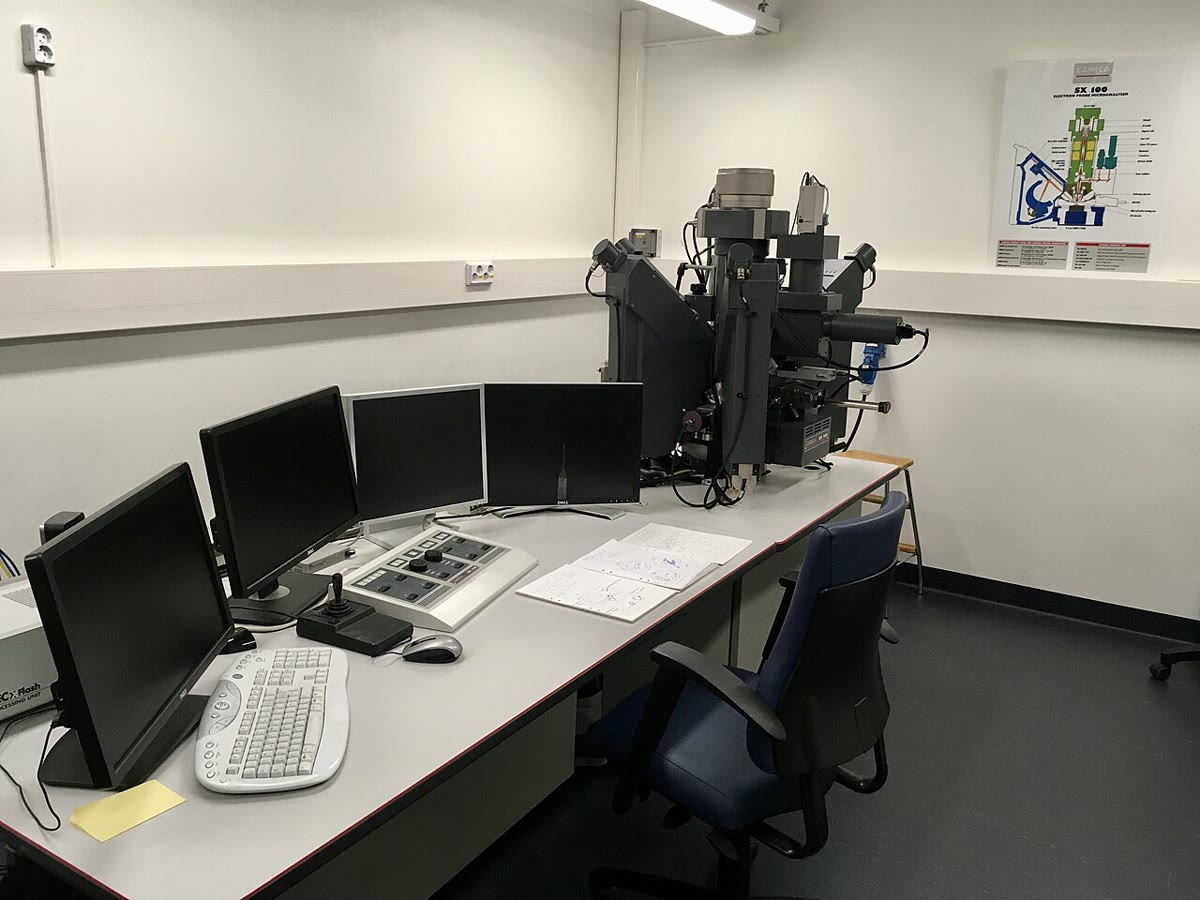
\includegraphics[width=\linewidth]{images/book4/b2-31-microprobe.jpg}
\par\smallskip{\scriptsize Une \omterm{def:b2:field-lab-methods-2:epma}{microsonde électronique} : la colonne électronique, avec ses spectromètres
autour, et le poste de l'opérateur. Photographie Kallerna, CC BY-SA 4.0 (Wikimedia Commons).}
\end{minipage}
\end{inthelab}
% ledger: sercE:epma-spot, sercE:coating, photo:b2-31-microprobe

\section{Analyse isotopique}\label{sec:b2:field-lab-methods-2:isotopes}

Les \omterm{def:b2:isotope-geochemistry:tracer}{traceurs isotopiques radiogéniques} et les âges (\cref{ch:b2:isotope-geochemistry}) reposent sur des rapports mesurés
à 0.01--\qty{0.001}{\percent} près, sur des éléments séparés de la roche par dissolution
et chromatographie d'échange d'ions dans un laboratoire propre, sous air filtré (typiquement classe 100 à
1000) afin que la poussière n'ajoute rien aux petites quantités analysées.
% ledger: sercT:tims

\begin{definition}[Spectrométrie de masse à thermo-ionisation, ICP-MS multicollecteur, biais de masse]\label{def:b2:field-lab-methods-2:tims}
Dans la \emph{spectrométrie de masse à thermo-ionisation}\index{spectrométrie de masse à thermo-ionisation} (TIMS), un
élément purifié est déposé sur un ruban métallique mince et ionisé par chauffage sous vide~; les ions
sont accélérés sous une tension pouvant atteindre \qty{10}{kV}, séparés par masse dans un secteur magnétique
et recueillis. Dans l'\emph{ICP-MS multicollecteur}\index{ICP-MS multicollecteur} les ions proviennent d'un
plasma à couplage inductif, qui ionise des éléments difficiles à ioniser thermiquement, et plusieurs
collecteurs mesurent simultanément les faisceaux de masses différentes. Le \emph{biais
de masse}\index{biais de masse} d'une mesure est l'écart entre le rapport isotopique mesuré et le
rapport vrai de l'échantillon, causé par l'instrument, qui transmet ou ionise plus facilement une masse
qu'une autre.
\end{definition}
% ledger: sercT:tims, sercM:mcicpms

Les deux instruments atteignent cette précision. Le TIMS ionise en général moins de
\qty{1}{\percent} des atomes, et son \omterm{def:b2:field-lab-methods-2:tims}{biais de masse} varie sans cesse au cours d'une série. Le biais est corrigé en fixant le rapport de deux isotopes que nulle
désintégration ne modifie, ce qui exige un élément ayant au moins trois isotopes, dont deux stables et non
radiogéniques. Pour le strontium, $^{86}\mathrm{Sr}/^{88}\mathrm{Sr}$ est fixé à 0.1194, et une forme courante
de la correction est la loi exponentielle.
% ledger: sercT:tims, sercM:mcicpms, cheong14:mass-bias, ciaaw:sr-isotopes

\begin{proposition}[Loi exponentielle du biais de masse]\label{prop:b2:field-lab-methods-2:bias}
Supposons que chaque rapport mesuré de deux isotopes de masses $m_i$ et $m_j$ soit relié au vrai
rapport par $R_{ij}^{\mathrm{true}} = R_{ij}^{\mathrm{meas}}\,(m_i/m_j)^{\beta}$, avec un seul exposant
$\beta$ pour toute la série. Alors le rapport mesuré $r$ d'un couple de référence, dont la valeur vraie
$r_0$ est connue, donne
\begin{equation}
\beta = \frac{\ln(r_0/r)}{\ln(m_k/m_l)}
\label{eq:b2:field-lab-methods-2:beta}
\end{equation}
pour le couple de référence $k/l$, et chaque autre rapport est corrigé avec le même $\beta$.
\end{proposition}

\begin{proof}
Appliquée au couple de référence, la loi s'écrit $r_0 = r\,(m_k/m_l)^\beta$~; en prenant les logarithmes,
$\ln(r_0/r) = \beta\ln(m_k/m_l)$, soit \eqref{eq:b2:field-lab-methods-2:beta}. L'exposant est
commun à tous les rapports de la série par hypothèse, il corrige donc chacun d'eux.
\end{proof}

Pour le strontium, le couple de référence est $^{86}\mathrm{Sr}/^{88}\mathrm{Sr}$ avec $r_0 = 0.1194$, et
le rapport corrigé $^{87}\mathrm{Sr}/^{86}\mathrm{Sr}$ vaut le rapport mesuré multiplié par
$(m_{87}/m_{86})^\beta$. Les abondances de la CIAAW, \qty{9.86}{\percent} du strontium 86 et
\qty{82.58}{\percent} du strontium 88, donnent la même valeur. Chaque série comporte aussi un \omterm{def:b2:isotope-geochemistry:standards}{étalon isotopique
de référence}~: un laboratoire a mesuré $^{87}\mathrm{Sr}/^{86}\mathrm{Sr} = 0.710252 \pm
0.000007$ sur le matériau de référence NBS~987 en sept séries.
% ledger: cheong14:mass-bias, ciaaw:sr-isotopes

Les rapports seuls ne donnent pas une concentration. Pour cela, une quantité connue d'un \emph{spike}, solution de
l'élément artificiellement enrichi en un isotope, est mélangée à l'échantillon dissous avant la chimie, et le rapport
est mesuré dans le mélange. Les laboratoires TIMS l'utilisent à la fois pour les
concentrations et pour les rapports parent-fille.
% ledger: sercT:tims

\begin{proposition}[Dilution isotopique]\label{prop:b2:field-lab-methods-2:id}
Soit un échantillon contenant $N_x$ moles d'un isotope de référence $b$ et un spike contenant $N_s$ moles de celui-ci, et soient
$R_x$, $R_s$ et $R_m$ les rapports d'un second isotope $a$ à $b$ dans l'échantillon, le spike et
le mélange. Alors
\begin{equation}
N_x = N_s\,\frac{R_s - R_m}{R_m - R_x} .
\label{eq:b2:field-lab-methods-2:id}
\end{equation}
Une erreur relative $\varepsilon$ sur $R_m$ donne à $N_x$ l'erreur relative $\mathcal{M}\varepsilon$,
avec le facteur d'amplification de l'erreur
\begin{equation}
\mathcal{M} = \frac{R_m\,(R_s - R_x)}{(R_s - R_m)(R_m - R_x)} ,
\label{eq:b2:field-lab-methods-2:mag}
\end{equation}
qui est minimal lorsque $R_m = \sqrt{R_s R_x}$.
\end{proposition}
\index{dilution isotopique}

\begin{proof}
L'isotope $a$ se conserve au mélange~: $R_m(N_x + N_s) = R_x N_x + R_s N_s$, donc $N_x(R_m - R_x) =
N_s(R_s - R_m)$, soit \eqref{eq:b2:field-lab-methods-2:id}. Sa dérivée logarithmique est
$\mathrm{d}\ln N_x/\mathrm{d}\ln R_m = R_m\,[-1/(R_s - R_m) - 1/(R_m - R_x)] = -\mathcal{M}$, avec
$\mathcal{M}$ comme dans \eqref{eq:b2:field-lab-methods-2:mag}. À la constante positive $R_s - R_x$ près,
$1/\mathcal{M} = (R_s - R_m)(R_m - R_x)/R_m = R_s + R_x - R_m - R_sR_x/R_m$, dont la dérivée
$-1 + R_sR_x/R_m^2$ s'annule en $R_m = \sqrt{R_sR_x}$, maximum de $1/\mathcal{M}$.
\end{proof}

La \omterm{prop:b2:field-lab-methods-2:id}{dilution isotopique} n'a besoin ni d'une droite d'étalonnage ni d'une récupération complète de l'élément au cours de
la chimie~: une fois le spike et l'échantillon mélangés, les pertes affectent les deux de la même façon. Un spike de strontium publié
par exemple, contient \qty{99.65}{\percent} de strontium 84, avec
$^{84}\mathrm{Sr}/^{88}\mathrm{Sr} = 561.4$ et $^{86}\mathrm{Sr}/^{88}\mathrm{Sr} = 0.7661$, à
\qty{15.271}{\micro\gram} de strontium par gramme de solution. Son rapport 86/88 montre pourquoi le \omterm{def:b2:field-lab-methods-2:tims}{biais de
masse} d'un mélange avec spike ne peut pas être corrigé en fixant $^{86}\mathrm{Sr}/^{88}\mathrm{Sr}$ à sa
valeur naturelle~: le spike a déplacé ce rapport.
% ledger: cheong14:spike, cheong14:mass-bias

\section{Une campagne de cartographie sur la boutonnière de Varden}\label{sec:b2:field-lab-methods-2:campaign}

Au cœur de l'anticlinal de Varden, l'érosion a entaillé la couverture gréseuse et mis à nu le socle~: un schiste
intrudé par un granite. Une campagne destinée à alimenter le laboratoire commence sur le terrain. Deux profils
sont parcourus d'ouest en est à travers la boutonnière, avec une station tous les
\qty{100}{m}~; à chacune, on note l'unité, et des échantillons frais sont prélevés là où la roche n'est pas altérée,
numérotés avec la station et, lorsque les fabriques doivent être mesurées, orientés. La figure montre ce que
rencontrent les stations~: sur les 30, dix sont sur le granite, dix sur la couverture gréseuse, une sur le schiste,
une sur le calcaire et huit sur les alluvions du fond de vallée, où aucune roche
n'affleure.

\begin{omfigure}
\centering
\begin{tikzpicture}
\begin{axis}[axis equal image, xmin=2.4, xmax=4.6, ymin=3.1, ymax=5.0, width=0.66\linewidth,
  tick label style={font=\scriptsize}, xlabel={est (km)}, ylabel={nord (km)},
  label style={font=\small}]
% units: figdata/shared/region.py (read only); stations: figdata/bachelor-2/labmethods.py part stations
\addplot[lith schist, draw=black, line width=0.3pt, even odd rule] table {figdata/out/shared-region-unit-schist.dat};
\addplot[lith granite, draw=black, line width=0.3pt, even odd rule] table {figdata/out/shared-region-unit-granite.dat};
\addplot[om lith={icsTriassic!35}{om sand}, draw=black, line width=0.3pt, even odd rule] table {figdata/out/shared-region-unit-sandstone.dat};
\addplot[om lith={icsJurassic!40}{om limestone}, draw=black, line width=0.3pt, even odd rule] table {figdata/out/shared-region-unit-limestone.dat};
\addplot[om lith={icsJurassic!15}{om shale}, draw=black, line width=0.3pt, even odd rule] table {figdata/out/shared-region-unit-shale.dat};
\addplot[lith alluvium, draw=black, line width=0.3pt, even odd rule] table {figdata/out/shared-region-unit-alluvium.dat};
\addplot[river] table {figdata/out/shared-region-river.dat};
\addplot[only marks, mark=*, mark size=1.6pt, mark options={fill=white, draw=black}]
  table[x=x_km, y=y_km] {figdata/out/bachelor-2-labmethods-stations.dat};
\addplot[only marks, mark=*, mark size=1.6pt, mark options={fill=omThm, draw=black},
  x filter/.expression={\thisrow{unit}==2 ? x : nan}]
  table[x=x_km, y=y_km] {figdata/out/bachelor-2-labmethods-stations.dat};
\node[font=\scriptsize, fill=white, inner sep=1pt, anchor=east] at (axis cs:2.76,3.7) {1};
\node[font=\scriptsize, fill=white, inner sep=1pt, anchor=west] at (axis cs:4.24,3.7) {15};
\node[font=\scriptsize, fill=white, inner sep=1pt, anchor=east] at (axis cs:2.76,4.4) {16};
\node[font=\scriptsize, fill=white, inner sep=1pt, anchor=west] at (axis cs:4.24,4.4) {30};
\draw[black, line width=0.5pt] (axis cs:3.5,4.44) -- (axis cs:3.5,4.62);
\node[font=\scriptsize, fill=white, inner sep=1pt, anchor=south] at (axis cs:3.5,4.62) {station~23};
\pic at (axis cs:4.45,4.75) {northarrow};
\end{axis}
\end{tikzpicture}
\par\smallskip{\small La boutonnière de socle des collines de Varden avec les 30 stations de deux profils ouest--est
espacés de \qty{100}{m}. Points rouges : stations sur le granite. Rose avec croix : granite~; gris : schiste~; violet : grès triasique~;
bleu : calcaire jurassique~; bleu pâle : schiste jurassique~; crème : alluvions de la rivière, qui
coule vers l'est. L'échantillon de granite du problème du week-end
provient de la station 23.}
\end{omfigure}

\begin{inthefield}[Échantillonner pour le laboratoire]
\centering
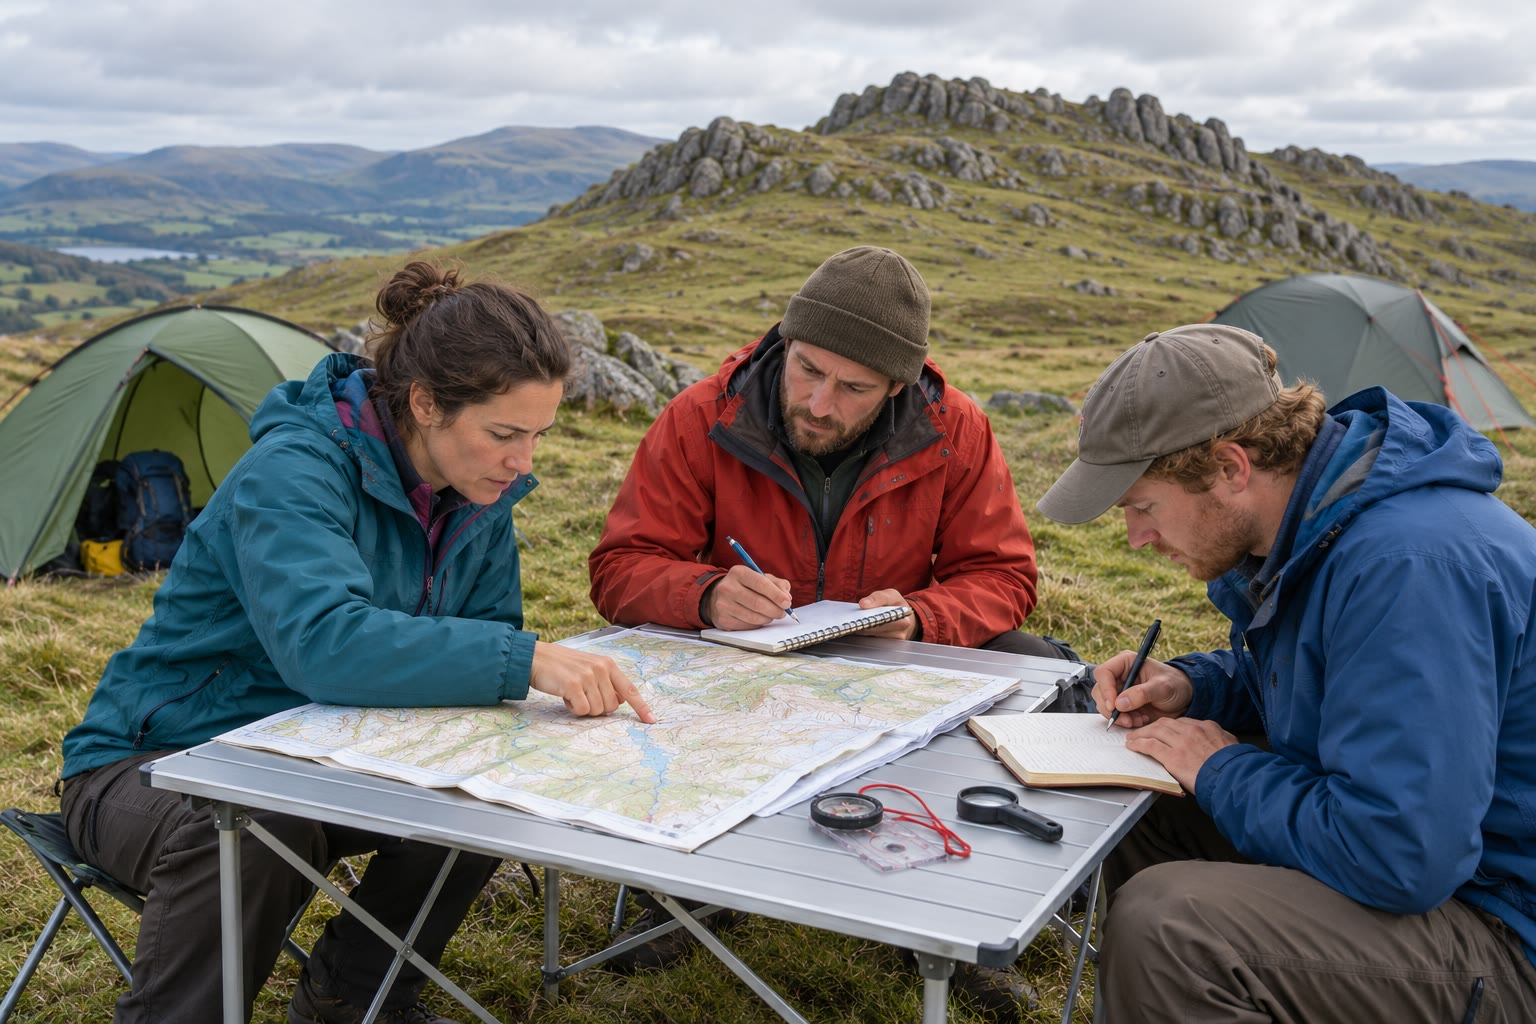
\includegraphics[width=0.56\linewidth]{images/book4/ai/b2-field-camp.jpg}
\par\smallskip{\small Une équipe de terrain prépare les profils du lendemain. Illustration générée par IA.}
\par\medskip\raggedright
Le soir, l'équipe reporte les stations sur la carte, vérifie que chaque numéro d'échantillon des carnets correspond
à un sac, et décide quels échantillons vont à quel laboratoire. Un échantillon de chaque unité va au laboratoire
de lames minces~; le granite et le schiste les plus frais vont
au broyage et à l'analyse de roche totale~; quelques échantillons de granite sont mis de côté pour les isotopes. Le
numéro de station suit chaque échantillon à travers chaque étape, du sac à la lame mince, à la poudre, à la perle et à la
ligne d'un tableau de données, si bien qu'un résultat aberrant peut être remonté jusqu'à son
affleurement.
\end{inthefield}

\section{La qualité d'un nombre}\label{sec:b2:field-lab-methods-2:quality}

Chaque étape de la chaîne ajoute sa propre erreur, et les méthodes de ce chapitre montrent les deux types que
distinguent les livres de chimie. Le \omterm{def:b2:field-lab-methods-2:modal}{comptage de points} et les rapports isotopiques ont surtout des erreurs aléatoires, qui
diminuent lorsque les comptages croissent, comme $1/\sqrt n$~; l'étalonnage a des erreurs systématiques, que la répétition ne
réduit pas et que seul un matériau de référence révèle. La figure des analyses de silice montre
les deux~: les barres sont la précision de la méthode, et un point qui s'écarte de zéro de plusieurs fois sa barre
divisée par la racine carrée du nombre d'analyses est un biais. Le même élément mesuré par deux
méthodes, le strontium par XRF et par \omterm{prop:b2:field-lab-methods-2:id}{dilution isotopique}, constitue un contrôle supplémentaire, puisque les deux n'ont
aucun étalonnage en commun. Les résultats sont donnés avec leur incertitude, arrondis à celle-ci, et avec les matériaux de
référence mesurés en même temps~; un nombre sans eux ne peut être comparé à aucun autre.

\section*{Exercices}\label{sec:b2:field-lab-methods-2:exercises}

Données pour les exercices, sauf mention contraire~: masses atomiques H 1.008, O 15.999, Mg 24.305, Al
26.982, Si 28.085, K 39.098, Sr 87.62~; masses isotopiques $^{86}\mathrm{Sr}$ 85.909261,
$^{87}\mathrm{Sr}$ 86.908878, $^{88}\mathrm{Sr}$ 87.905612~; strontium naturel
$^{84}\mathrm{Sr}/^{86}\mathrm{Sr} = 0.05680$, \qty{9.86}{\percent} de $^{86}\mathrm{Sr}$~; le spike
du texte, $^{84}\mathrm{Sr}/^{86}\mathrm{Sr} = 732.8$, \qty{0.13599}{\percent} de
$^{86}\mathrm{Sr}$, masse atomique 83.9242, \qty{15.271}{\micro\gram\per\gram}. Arrondir à trois
chiffres significatifs sauf mention contraire.
% ledger: ciaaw:H, ciaaw:O, ciaaw:Mg, ciaaw:Al, ciaaw:Si, ciaaw:K, ciaaw:sr-isotopes, cheong14:spike

\begin{exercise}[$\star$]\label{exo:b2:field-lab-methods-2:1}
(a) Nommer la texture ou le cristal~: (i) une dolérite dans laquelle les lattes de plagioclase sont entièrement enfermées dans
de grands cristaux d'augite~; (ii) un marbre à grains de calcite de taille égale dont les joints droits se rejoignent par
trois~; (iii) un cristal de staurotide long de \qty{5}{mm}, bourré d'inclusions de quartz dans un schiste à mica~;
(iv) un grenat entouré d'une bordure continue de plagioclase et de pyroxène. (b) Trois joints de grains
se rejoignent sous \ang{104}, \ang{128} et \ang{128}. Trouver le rapport de la tension du joint opposé à
l'angle de \ang{104} à celle des deux autres.
\end{exercise}

\begin{exercise}[$\star$]\label{exo:b2:field-lab-methods-2:2}
Une roche grenue contient \qty{25}{\percent} de quartz, 15 de feldspath alcalin, 40 de plagioclase, 12
de biotite, 8 de hornblende. (a) Recalculer Q, A et P. (b) Trouver P/(A+P) et nommer la roche. (c) Trouver
son indice de couleur et le qualifier.
\end{exercise}

\begin{exercise}[$\star$]\label{exo:b2:field-lab-methods-2:3}
Un comptage de 800 points trouve un minéral à \qty{12}{\percent}. (a) Trouver l'écart type de
cette proportion, et sa valeur relative. (b) Quelle serait-elle avec 3200 points~?
\end{exercise}

\begin{exercise}[$\star$]\label{exo:b2:field-lab-methods-2:4}
Une poudre de \qty{0.8000}{g} pèse \qty{0.7712}{g} après calcination, et le résidu est fondu avec
\qty{8.0000}{g} de fondant. (a) Trouver la \omterm{def:b2:field-lab-methods-2:xrf}{perte au feu}. (b) Trouver la fraction massique de l'échantillon dans
la perle. (c) Le verre contient \qty{5.20}{\percent} \ce{SiO2}. Trouver la silice de la poudre calcinée
et de la poudre d'origine.
\end{exercise}

\begin{exercise}[$\star\star$]\label{exo:b2:field-lab-methods-2:5}
(a) Combien de points faut-il pour mesurer un minéral accessoire constituant \qty{2}{\percent} d'une roche
avec une erreur standard relative de \qty{10}{\percent}~? (b) Et un minéral constituant \qty{30}{\percent},
avec la même erreur relative~? (c) Commenter l'effort qu'exige un minéral rare.
\end{exercise}

\begin{exercise}[$\star\star$]\label{exo:b2:field-lab-methods-2:6}
Dans les résultats USGS de la figure, la rhyolite RGM-1 a donné \ce{SiO2} $= 72.89$ avec un écart type
de 0.19 sur 20 analyses (valeur recommandée 73.45), et le basalte BCR-2 a donné 54.17 avec 0.13 sur
20 analyses (valeur recommandée 54.1). (a) Trouver le taux de recouvrement de chacun, en pour cent. (b) Trouver l'écart type
de chaque moyenne, et exprimer chaque écart à la valeur recommandée en unités de celui-ci.
(c) Quel résultat révèle un biais~? La méthode est-elle moins précise pour RGM-1~?
\end{exercise}

\begin{exercise}[$\star\star$]\label{exo:b2:field-lab-methods-2:7}
Une analyse à la microsonde d'une phlogopite pure, $\mathrm{KMg_3AlSi_3O_{10}(OH)_2}$, est à vérifier.
(a) Trouver la masse molaire de la formule et la fraction massique de \ce{H2O} qu'elle contient. (b) Trouver les
fractions massiques de \ce{K2O}, \ce{MgO}, \ce{Al2O3} et \ce{SiO2}, ainsi que le total qu'une analyse exacte donnerait~:
(c) Pourquoi un total d'environ \qty{96}{\percent} pour un mica n'est-il pas une mauvaise analyse~?
\end{exercise}

\begin{exercise}[$\star\star$]\label{exo:b2:field-lab-methods-2:8}
Une série TIMS sur un étalon de strontium donne $^{86}\mathrm{Sr}/^{88}\mathrm{Sr} = 0.11905$ et
$^{87}\mathrm{Sr}/^{86}\mathrm{Sr} = 0.71062$. (a) Trouver l'exposant $\beta$ de la loi exponentielle.
(b) Corriger le rapport $^{87}\mathrm{Sr}/^{86}\mathrm{Sr}$, à cinq décimales. (c) L'isotope léger ou
l'isotope lourd était-il favorisé dans la série~?
\end{exercise}

\begin{exercise}[$\star\star$]\label{exo:b2:field-lab-methods-2:9}
Pour vérifier sa \omterm{prop:b2:field-lab-methods-2:id}{dilution isotopique}, un laboratoire ajoute du spike à \qty{0.0500}{g} du basalte de référence BHVO-2
avec \qty{0.1000}{g} du spike du texte, et mesure $^{84}\mathrm{Sr}/^{86}\mathrm{Sr} =
0.874$ dans le mélange. (a) Trouver les moles de $^{86}\mathrm{Sr}$ dans la prise de spike. (b) Trouver les
moles de $^{86}\mathrm{Sr}$ dans l'échantillon, et sa concentration en strontium en ppm. (c) Comparer à
la valeur recommandée de \qty{394.1}{ppm}.
\end{exercise}

\begin{exercise}[$\star\star\star$]\label{exo:b2:field-lab-methods-2:10}
Pour le spike de strontium du texte ($R_s = 732.8$, $R_x = 0.05680$)~: (a) trouver le rapport du mélange
qui minimise le facteur d'amplification de l'erreur, et sa valeur en ce point~; (b) évaluer $\mathcal M$ en
$R_m = 0.1$, 0.5, 1.664 et 100~; (c) expliquer pourquoi un mélange proche de l'un ou l'autre pôle est à
éviter, et quelle latitude l'analyste a en pratique.
\end{exercise}

\begin{exercise}[$\star\star\star$]\label{exo:b2:field-lab-methods-2:11}
Un comptage dans un granite trouve 400 points de feldspath, dont \qty{62}{\percent} de plagioclase. (a) En traitant le
plagioclase parmi les points de feldspath comme un comptage binomial, trouver l'écart type de
P/(A+P). (b) À quelle distance du seuil de la granodiorite se situe le résultat, en écarts types~? (c) Combien
de points de feldspath le placeraient à deux écarts types du seuil~?
\end{exercise}

\begin{exercise}[$\star\star\star$]\label{exo:b2:field-lab-methods-2:12}
Un minéral occupe une fraction $p$ d'une roche. (a) Montrer que la probabilité que $n$ points indépendants
manquent tous ce minéral est $(1-p)^n$. (b) Combien de points donnent une probabilité d'au moins \qty{95}{\percent}
de toucher au moins une fois un minéral constituant \qty{1}{\percent} de la roche~? (c) Même question pour le zircon à
\qty{0.05}{\percent}, et conclure sur la façon de rechercher un minéral accessoire.
\end{exercise}

\section*{Problème du week-end}

\begin{problem}[{Problème du week-end --- De l'affleurement à l'analyse}]\label{pb:b2:field-lab-methods-2:1}
% invented sample; data: ledger rows below; values: calc/ch31.py
L'échantillon VH-23 du granite de Varden a été prélevé à la station 23 de la campagne. Une lame mince a été
comptée par points sur une grille régulière de 1200 points~: quartz 372, feldspath alcalin 348, plagioclase 324,
biotite 108, muscovite 36, oxydes opaques 12. Une poudre de \qty{0.8000}{g} a pesé \qty{0.7949}{g}
après calcination à \qty{925}{\celsius} et a été fondue avec \qty{8.0000}{g} de fondant. Des perles de trois
matériaux de référence ont donné ces intensités en \ce{SiO2} (milliers de coups par seconde, kcps)~: BCR-2,
recommandée \qty{54.1}{\percent}, 21.66~; AGV-2, 59.3, 23.70~; RGM-1, 73.45, 29.37~; la perle de granite
a donné 28.63. Les autres oxydes du granite totalisent \qty{27.15}{\percent}. Pour les isotopes,
\qty{0.1000}{g} de poudre de l'échantillon ont été dissous et mélangés à \qty{0.2500}{g} du spike du texte~;
l'échantillon est supposé avoir les abondances naturelles du strontium des exercices. Utiliser les données des
exercices.

\noindent\textbf{Partie I --- La composition modale.}
\begin{enumerate}
  \item Trouver la proportion modale de chaque minéral.
  \item Trouver l'écart type de la proportion de quartz, et l'écart type relatif
        de la proportion de muscovite.
  \item Trouver $M$ et l'indice de couleur $M'$, et qualifier la roche.
  \item Recalculer Q, A et P à une somme de 100.
  \item Trouver P/(A+P) et nommer la roche sur le \omterm{def:b2:magmatic-series:qapf}{diagramme QAPF}.
  \item Avec l'écart type binomial de P/(A+P) sur les 672 points de feldspath, le nom est-il
        sûr~?
  \item Combien de points faudrait-il pour ramener l'écart type de la proportion de quartz à un
        point de pourcentage~?
\end{enumerate}

\noindent\textbf{Partie II --- Silice par fluorescence X.}
\begin{enumerate}[resume]
  \item Trouver la \omterm{def:b2:field-lab-methods-2:xrf}{perte au feu}.
  \item Trouver la fraction massique de l'échantillon dans la perle, et la silice du verre si la
        poudre calcinée contient \qty{72}{\percent}.
  \item Ajuster la droite des moindres carrés $c = aI + b$ à travers les trois matériaux de référence~; donner $a$ à
        quatre décimales et $b$ à deux.
  \item Trouver le \ce{SiO2} du granite, à deux décimales.
  \item Trouver les résidus des trois matériaux de référence. La droite est-elle adéquate~?
  \item Additionner les oxydes et la \omterm{def:b2:field-lab-methods-2:xrf}{perte au feu}. La procédure USGS reprendrait-elle cette analyse~?
  \item Recalculer la silice à une somme de 100 sans les composés volatils.
\end{enumerate}

\noindent\textbf{Partie III --- Biais de masse.}
\begin{enumerate}[resume]
  \item À partir des abondances de la CIAAW, trouver le $^{86}\mathrm{Sr}/^{88}\mathrm{Sr}$ naturel et le comparer
        à la valeur utilisée pour la normalisation.
  \item Une prise non spikée donne $^{86}\mathrm{Sr}/^{88}\mathrm{Sr} = 0.11853$. Trouver $\beta$ à
        quatre décimales.
  \item Elle donne $^{87}\mathrm{Sr}/^{86}\mathrm{Sr} = 0.71655$. La corriger, à cinq décimales.
  \item Trouver le biais par unité de masse, en pour cent.
  \item Pourquoi cette correction ne peut-elle pas être faite sur le mélange avec spike de la partie IV~?
\end{enumerate}

\noindent\textbf{Partie IV --- Dilution isotopique.}
\begin{enumerate}[resume]
  \item Vérifier que le spike contient \qty{99.65}{\percent} de strontium 84 et \qty{0.13599}{\percent}
        de strontium 86.
  \item Trouver les moles de strontium et de $^{86}\mathrm{Sr}$ dans la prise de spike, à quatre
        chiffres significatifs.
  \item Vérifier les valeurs $R_s = 732.8$ et $R_x = 0.05680$ des exercices.
  \item Le rapport corrigé du mélange est $R_m = 1.6812$. Trouver les moles de $^{86}\mathrm{Sr}$
        de l'échantillon.
  \item Trouver le facteur d'amplification de l'erreur. Avec $R_m$ connu à \qty{0.01}{\percent} près et la concentration
        du spike à $\pm\qty{0.031}{\micro\gram\per\gram}$, trouver l'incertitude relative du
        résultat.
  \item Trouver la concentration en strontium du granite de Varden, en ppm.
\end{enumerate}
\end{problem}
% ledger: bgsI:qapf, bgsI:colour-index, usgsT:procedure, usgsT:sio2-table, ciaaw:sr-isotopes, cheong14:spike, cheong14:mass-bias
